\section{BITS函数实验与分析}
\begin{center}
    每题8分,总分不超过80分
    截图:  \$ ./btest –f 函数名
\end{center}

\subsection{函数lsbZero的实现及说明}

\paragraph{程序如下:}
\begin{lstlisting}[language = c]
int lsbZero(int x) {
	return x & ((1 << 31) >> 30);
}
\end{lstlisting}

\begin{figure}[H]
\begin{minipage}[c]{0.5\linewidth}
\paragraph{设计思想:}主要考虑获得0xfffffffe,即处lsb为0外,其他位全部为1的值与x相与。
\end{minipage}
\begin{minipage}[c]{0.4\linewidth}
\centering
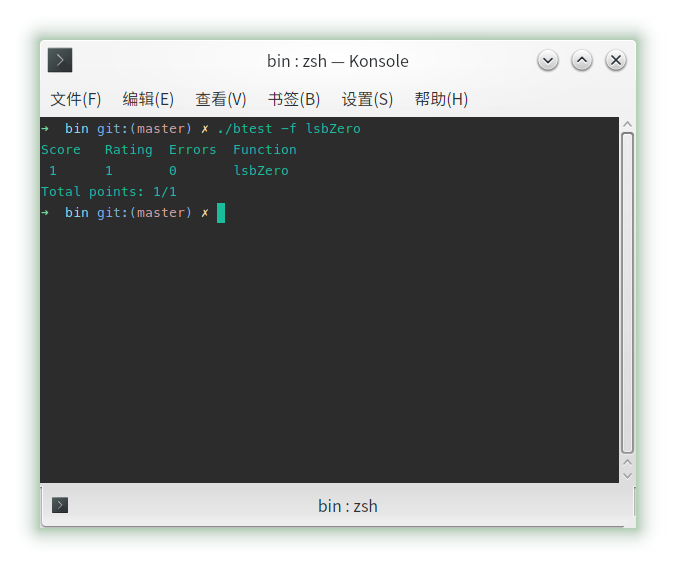
\includegraphics[width=0.9\linewidth]{figures/lsbZero}
\caption{btest截图-lsbZero}
\label{fig:lsbzero}
\end{minipage}
\end{figure}

\subsection{函数byteNot的实现及说明}

\textbf{程序如下:}
\begin{lstlisting}[language = c]
int byteNot(int x, int n) {
	return x ^ (0xFF << (n << 3));
}
\end{lstlisting}

\begin{figure}[H]
\begin{minipage}[c]{0.5\linewidth}
\textbf{设计思想:}发现数值与1异或可以取反,将需要取反的字节的与0xff对齐进行异或即可。	
\end{minipage}
\begin{minipage}[c]{0.4\linewidth}
\centering
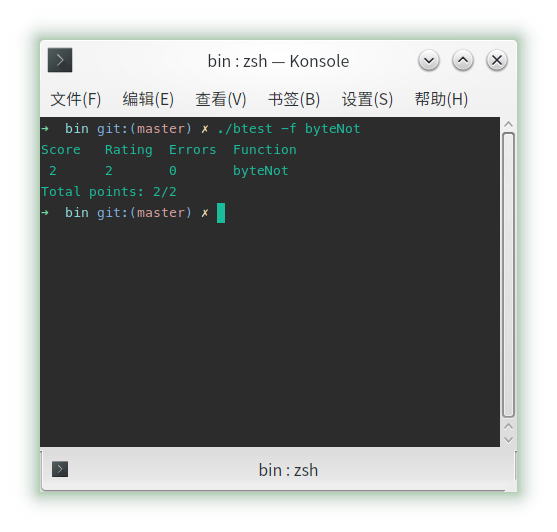
\includegraphics[width=0.9\linewidth]{figures/byteNot}
\caption{btest截图-byteNot}
\label{fig:byteNote}
\end{minipage}
\end{figure}

\subsection{函数byteXor的实现及说明}

\textbf{程序如下:}
\begin{lstlisting}[language = c]
int byteXor(int x, int y, int n) {
	return !(!(0xFF & ((x ^ y) >> (n << 3))));
}
\end{lstlisting}

\begin{figure}[H]
\begin{minipage}[c]{0.5\linewidth}
		
\textbf{设计思想:}简单考虑,对所有位进行异或比较,然后取得所需要的字节部分的结果即可,使用两次逻辑取非,获得逻辑值。
		
\end{minipage}
\begin{minipage}[c]{0.4\linewidth}
\centering
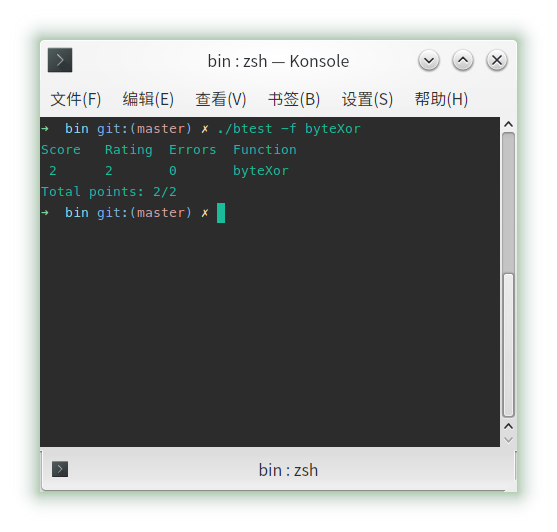
\includegraphics[width=0.9\linewidth]{figures/byteXor}
\caption{btest截图-byteXor}
\label{fig:byteXor}
\end{minipage}
\end{figure}

\subsection{函数logicalAnd的实现及说明}
\textbf{程序如下:}
\begin{lstlisting}[language = c]
int logicalAnd(int x, int y) {
	return !(!x | !y);
}
\end{lstlisting}

\begin{figure}[H]
\begin{minipage}[c]{0.5\linewidth}
\textbf{设计思想:}使用逻辑非取得输入值的逻辑值,再进行位运算即可获得逻辑结果。
		
\end{minipage}
\begin{minipage}[c]{0.4\linewidth}
\centering
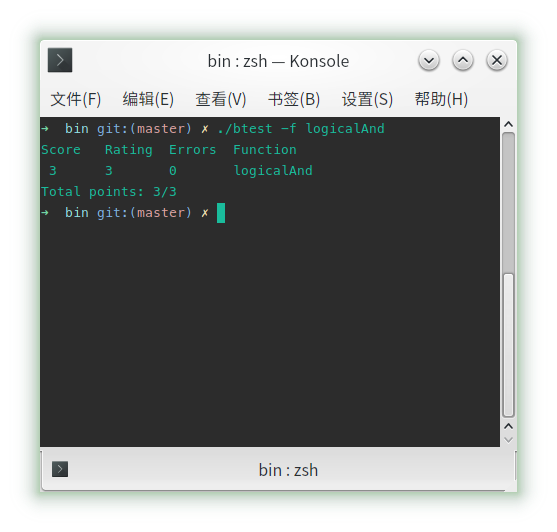
\includegraphics[width=0.9\linewidth]{figures/logicalAnd}
\caption{btest截图-logicalAnd}
\label{fig:logicalAnd}
\end{minipage}
\end{figure}

\subsection{函数logicalOr的实现及说明}
\textbf{程序如下:}

\begin{lstlisting}[language = c]
int logicalOr(int x, int y) {
	return !(!x & !y);
}
\end{lstlisting}

\begin{figure}[H]
\begin{minipage}[c]{0.5\linewidth}
\textbf{设计思想:}使用逻辑非取得输入值的逻辑值,再进行位运算即可获得逻辑结果。
		
\end{minipage}
\begin{minipage}[c]{0.4\linewidth}
\centering
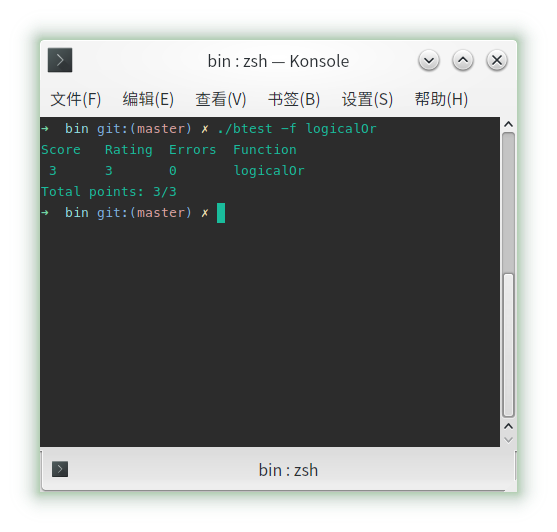
\includegraphics[width=0.9\linewidth]{figures/logicalOr}
\caption{btest截图-logicalOr}
\label{fig:logicalOr}
\end{minipage}
\end{figure}

\subsection{函数rotateLeft的实现及说明}
\textbf{程序如下:}
	
\begin{lstlisting}[language = c]
int rotateLeft(int x, int n) {
    int N_31 = ~n + 33;
	return (x << n) | ((~0u >> N_31) & (x >> N_31));
}
\end{lstlisting}
	
\begin{figure}[H]
\begin{minipage}[c]{0.5\linewidth}
\textbf{设计思想:}重点是发现 \lstinline[language=c]|-a=~a+1|,之后将数据位进行移动,使用掩码做多余数据消除,而后合并。
\end{minipage}
\begin{minipage}[c]{0.4\linewidth}
\centering
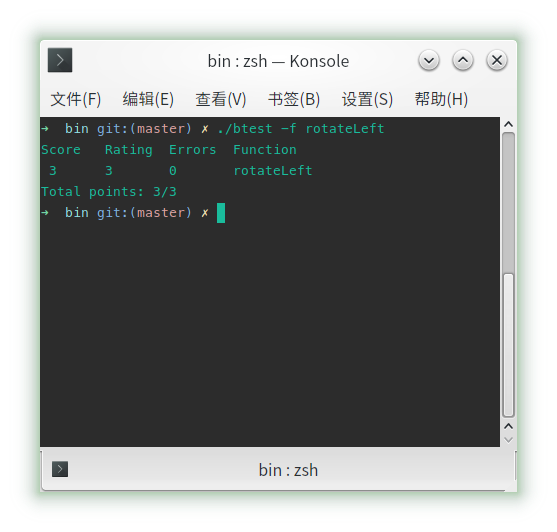
\includegraphics[width=0.9\linewidth]{figures/rotateLeft}
\caption{btest截图-rotateLeft}
\label{fig:rotateLeft}
\end{minipage}
\end{figure}

\subsection{函数parityCheck的实现及说明}

\textbf{程序如下:}

\begin{lstlisting}[language = c]
int parityCheck(int x) {
    x = (x >> 16) ^ x;
    x = (x >> 8) ^ x;
    x = (x >> 4) ^ x;
    x = (x >> 2) ^ x;
    x = (x >> 1) ^ x;
    return x & 0x01;
}
\end{lstlisting}

\begin{figure}[H]
    \begin{minipage}[c]{0.5\linewidth}
        \textbf{设计思想:}使用归并的思路进行各位的比较,若为偶数个1,最终会被全部抵消。
    \end{minipage}
    \begin{minipage}[c]{0.4\linewidth}
        \centering
        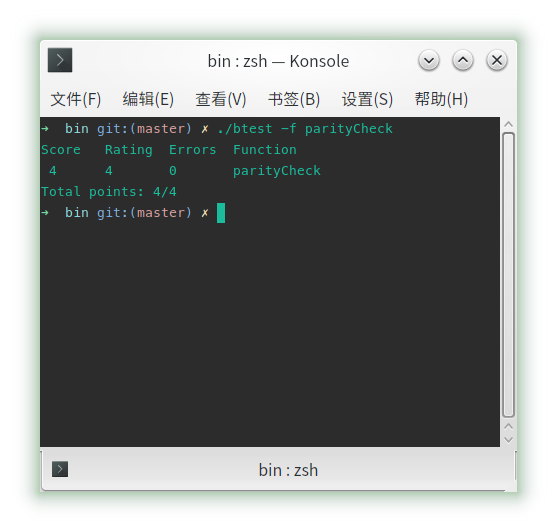
\includegraphics[width=0.9\linewidth]{figures/parityCheck}
        \caption{btest截图-parityCheck}
        \label{fig:parityCheck}
    \end{minipage}
\end{figure}

\subsection{函数mul2OK的实现及说明}
\textbf{程序如下:}

\begin{lstlisting}[language = c]
int mul2OK(int x) {
	return !(0x01 & ((x >> 31) ^ (x >> 30)));
}
\end{lstlisting}

\begin{figure}[H]
\begin{minipage}[c]{0.5\linewidth}
\textbf{设计思想:}主要是判断符号位是否发生了改变,若发生则是发生了溢出。
\end{minipage}
\begin{minipage}[c]{0.4\linewidth}
\centering
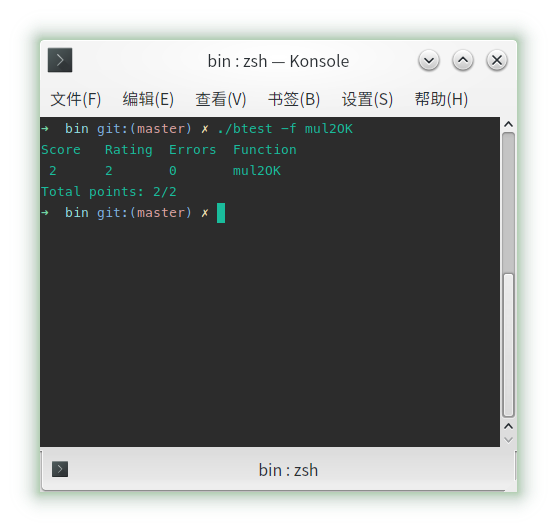
\includegraphics[width=0.9\linewidth]{figures/mul2OK}
\caption{btest截图-mul2OK}
\label{fig:mul2OK}
\end{minipage}
\end{figure}

\subsection{函数mult3div2的实现及说明}
\begin{lstlisting}[language = c]
int mult3div2(int x) {
    int xmult3 = (x << 1) + x;
    return (xmult3 >> 1) + (((xmult3 >> 31) & 1) & (((xmult3 << 31) >> 31) & 1));
}
\end{lstlisting}

\begin{figure}[H]
    \begin{minipage}[c]{0.5\linewidth}
        \textbf{设计思想:}左移一位再加$x$即$x*3$,右移一位即得$(x*3)/2$,当$x*3$的最高位和最低位都为0时需要+1。
    \end{minipage}
    \begin{minipage}[c]{0.4\linewidth}
        \centering
        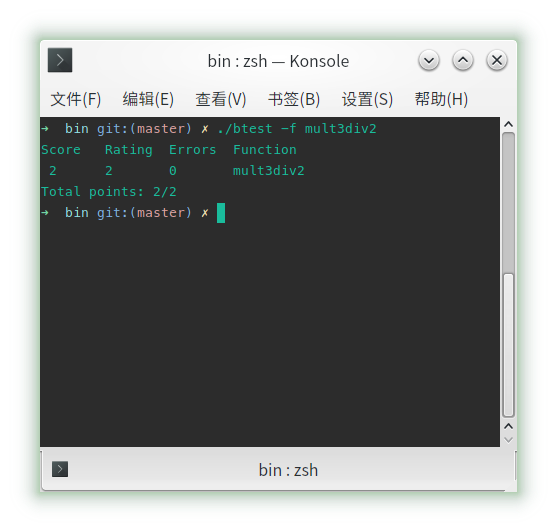
\includegraphics[width=0.9\linewidth]{figures/mult3div2}
        \caption{btest截图-mult3div2}
        \label{fig:mult3div2}
    \end{minipage}
\end{figure}

\subsection{函数subOK的实现及说明}

\begin{lstlisting}[language = c]
int subOK(int x, int y) {
  int samesign = ((x ^ y) >> 31) & 0x01;
  return !(samesign & ((((x + ~y + 1) ^ x) >> 31) & 0x01));
}
\end{lstlisting}

\begin{figure}[H]
    \begin{minipage}[c]{0.5\linewidth}
        \textbf{设计思想:}重点是注意到两个数符号相同时不会产生溢出,当符号不同时,减数的符号位参加运算则是发生了溢出。
    \end{minipage}
    \begin{minipage}[c]{0.4\linewidth}
        \centering
        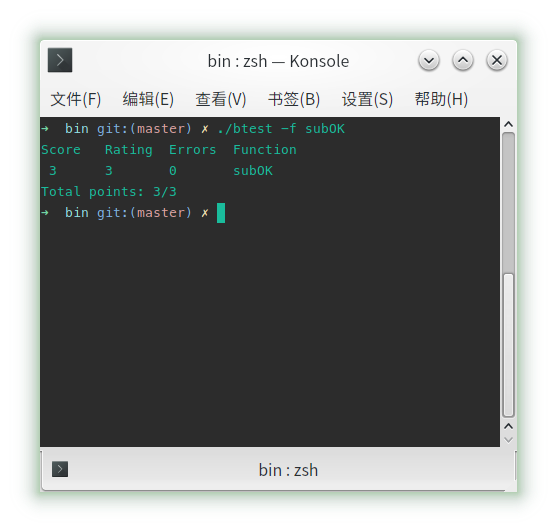
\includegraphics[width=0.9\linewidth]{figures/subOK}
        \caption{btest截图-subOK}
        \label{fig:subOK}
    \end{minipage}
\end{figure}

\subsection{函数absVal的实现及说明}
\textbf{程序如下:}

\begin{lstlisting}[language = c]
int absVal(int x) {
  return ((x >> 31) & (~(x - 1))) | (~(x >> 31) & x);
}
\end{lstlisting}

\begin{figure}[H]
\begin{minipage}[c]{0.5\linewidth}
\textbf{设计思想:}若为正则不做处理,若为负则进行\lstinline[language=c]|-a=~a+1|的逆运算,通过符号位的判断决定取得的值。
\end{minipage}
\begin{minipage}[c]{0.4\linewidth}
\centering
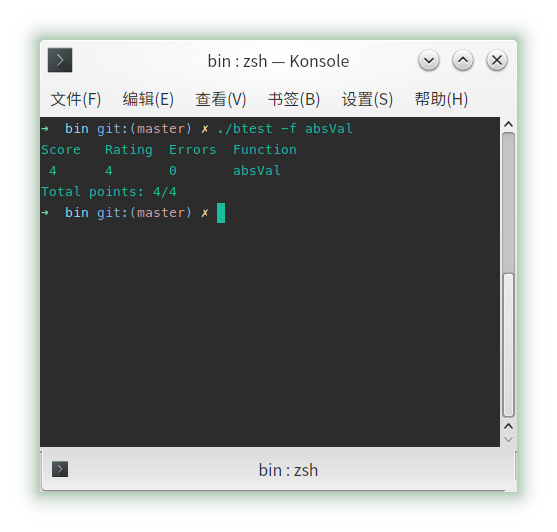
\includegraphics[width=0.9\linewidth]{figures/absVal}
\caption{btest截图-absVal}
\label{fig:absVal}
\end{minipage}
\end{figure}

\subsection{函数float\_abs的实现及说明}
\textbf{程序如下:}

\begin{lstlisting}[language = c]
unsigned float_abs(unsigned uf) {
	unsigned sign = uf >> 31;
	unsigned exp = uf >> 23 & 0xFF;
	unsigned frac = uf & 0x7FFFFF;
	return uf & 0x7fffffff | (sign * ((exp == 0xFF && frac) << 31));
}
\end{lstlisting}

\begin{figure}[H]
\begin{minipage}[c]{0.5\linewidth}
\textbf{设计思想:}符号位置零,若发现该数值为NaN则将符号位重新补上。
\end{minipage}
\begin{minipage}[c]{0.4\linewidth}
\centering
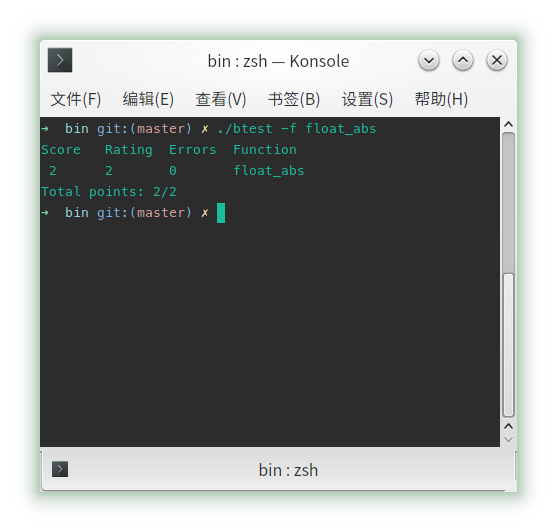
\includegraphics[width=0.9\linewidth]{figures/float_abs}
\caption{btest截图-float-abs}
\label{fig:float-abs}
\end{minipage}
\end{figure}

%\subsection{函数float\_f2i的实现及说明}
%\subsection{函数XXXX的实现及说明函数(CMU多出来的函数-不加分)}


